\section{実験装置}
\subsection{液体酸素(LOX)}
液体酸素(LOX)の基本的な物性値をTable2-1に、液体酸素の飽和蒸気圧と潜熱、密度を温度の関数としてそれぞれFig.2-およびFig.2-に示す。
\begin{figure}[htbp]
\centering
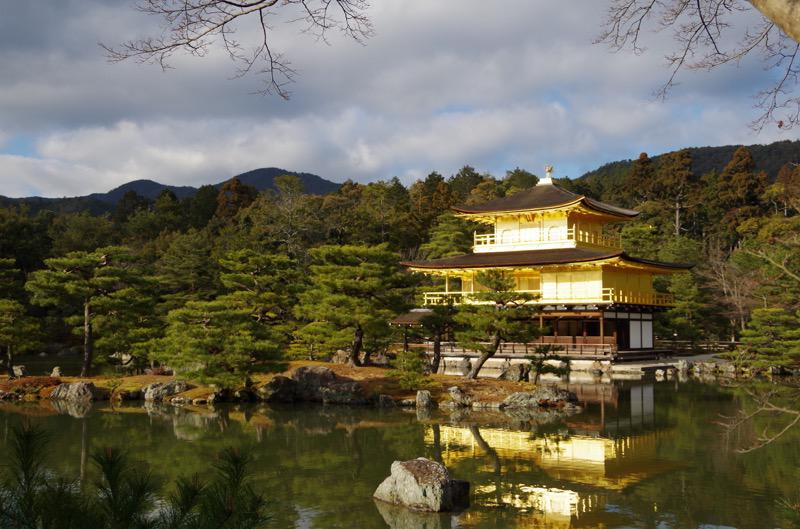
\includegraphics[width=10cm]{\FigAdd/apple.jpg}
\caption{TestPic}
\end{figure}
\subsection{アクリル樹脂(PMMA)}
本実験で用いる燃料はアクリル樹脂(PMMA)とした。アクリル樹脂の基本的な物性値をTable2-2に示す。

\subsection{プリバーナ方式液体酸素気化器}
本実験では2種類の気化器を使用した。
気化器1は気化器内部の状態を可視化するために、アクリル樹脂と石英ガラスを使用した。
気化器2は基礎データ取得のために、ステンレスとグラファイトを使用した。
各気化器の外観を図\ref{fig:Test1}に示す。
\begin{figure}
\centering
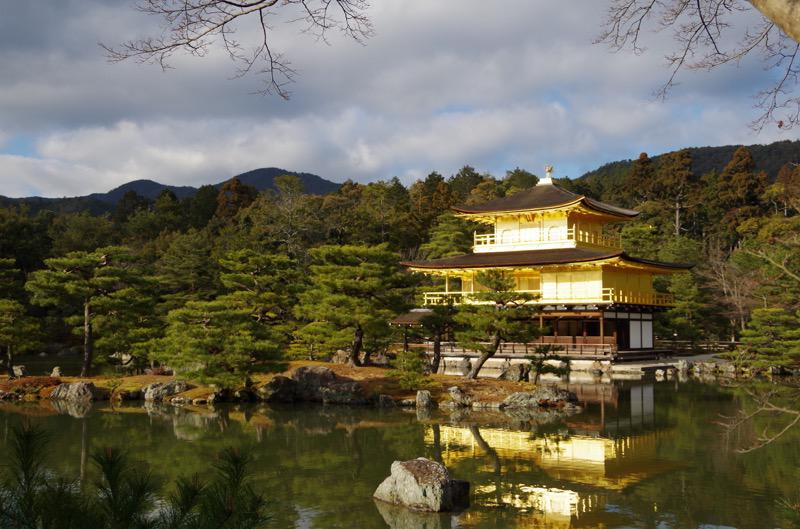
\includegraphics[width=5cm]{\FigAdd/apple.jpg}
\caption{TestPic}
\label{fig:Test1}
\end{figure}

\subsection{供給系}
本供給系は植松電機殿の設備を使用した。
LOXタンクの外観と概略図を図\ref{fig:LOXTankPho}、図\ref{fig:LOXTankPic}に示す。

\begin{figure}[htbp]
\begin{tabular}{cc}
\begin{minipage}{.5\textwidth}
\begin{center}
\centering
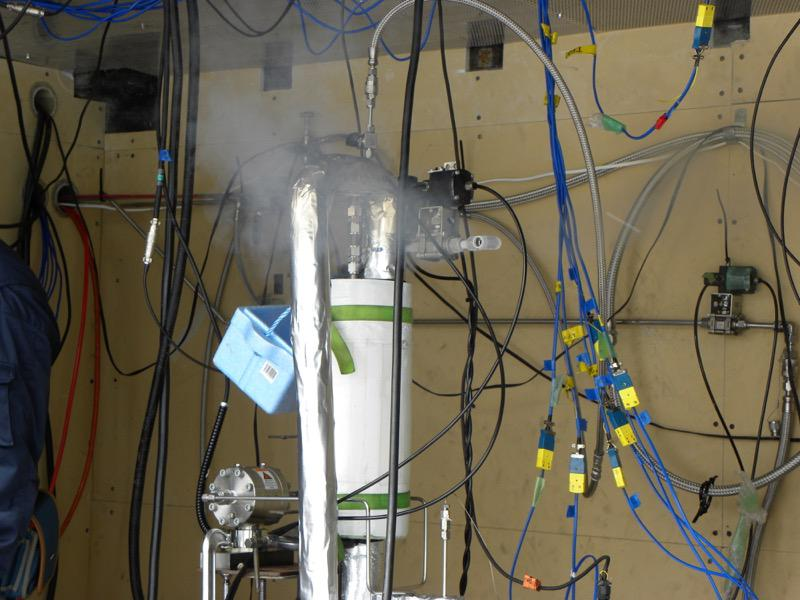
\includegraphics[width=6cm]{\FigAdd/LOXTankPic.jpg}
\caption{LOXタンク外観}
\label{fig:LOXTankPho}
\end{center}
\end{minipage}
\begin{minipage}{.5\textwidth}
\begin{center}
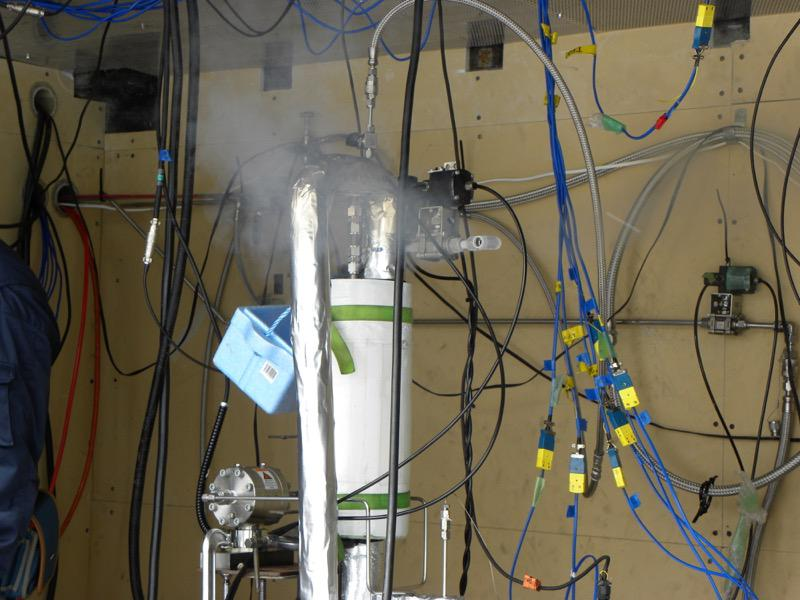
\includegraphics[width=6cm]{\FigAdd/LOXTankPic.jpg}
\caption{LOXタンク概略図}
\label{fig:LOXTankPic}
\end{center}
\end{minipage}
\end{tabular}
\end{figure}

本実験の外観をFig.2-に配管図をFig.2-を示す。
流量計測は

\begin{figure}[htbp]
\begin{tabular}{cc}
\begin{minipage}{.5\textwidth}
\begin{center}
\centering
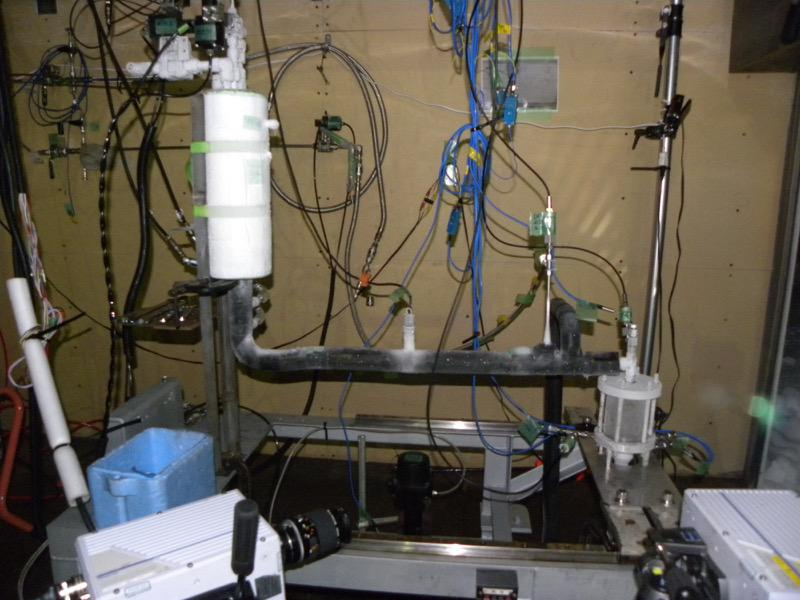
\includegraphics[width=6cm]{\FigAdd/LOXLinePic.jpg}
\caption{LOX供給系外観}
\label{fig:LOXLinePho}
\end{center}
\end{minipage}
\begin{minipage}{.5\textwidth}
\begin{center}
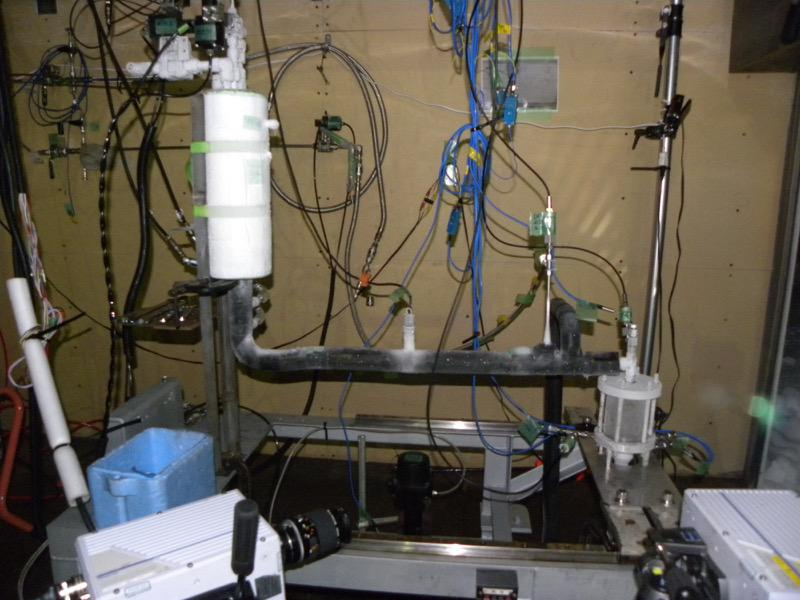
\includegraphics[width=6cm]{\FigAdd/LOXLinePic.jpg}
\caption{LOX配管図}
\label{fig:LOXLinePic}
\end{center}
\end{minipage}
\end{tabular}
\end{figure}


%\subsection{アクリル樹脂(PMMA)}
本実験で用いる燃料はアクリル樹脂(PMMA)とした。アクリル樹脂の基本的な物性値をTable2-2に示す。


